% chktex-file 44
\section{Экспериментальная часть}
\subsection{Описание установки}
Рентгенографические эксперименты проводились на монокристальном дифрактометре Bruker D8 Venture (см. рисунок~\ref{fig:D8_photo}).
Его оборудование и характеристики:
\begin{itemize}
    \item Микрофокусная трубка Incoatec $I \mu S \ 3.0$
    \begin{itemize}
        \item $\text{Cu} K\alpha$ и $\text{Mo} K\alpha$ излучение
        \item Монохроматизация и коллимация с помощью многослойных зеркал Монтеля
        \item Диаметр пучка $110\unit{мкм}$
        \item Расходимость $0.3\degree$
    \end{itemize}
    \item Двумерный детектором PHOTON III
    \begin{itemize}
        \item CMOS-технология матрицы
        \item Разрешение $768 \times 1024$ пикселей
        \item Размер пикселя $135 \times 135\unit{мкм}^2$
        \item Ручная установка расстояния до образца
    \end{itemize}
    \item Трехкружный гониометр FIXED-CHI
    \begin{itemize}
        \item Гониометр использует эйлерову геометрию
        \item Автоматическая регулировка углов $\varphi$ и $\omega$ для образца и $2\theta_D$ для детектора
        \item Угол $\chi$ фиксирован и равен $54.7112\degree$
        \item Воспроизводимость установки углов $0.0001\degree$
        \item Точность установки углов $0.005\degree$\footnote{Паспортная точность установки углов не указана, но согласно результатам измерения эталонного образца на порошковом дифрактометре Bruker D8 Advance, оснащенном аналогичным гониометром, она не хуже $0.005\degree$.}
    \end{itemize}
    \item Температурная приставка Oxford Cryostream 800Plus
    \begin{itemize}
            \item Стабильность поддержания температуры $0.2\unit{К}$
    \end{itemize}
    \item Управление прибором средствами программного пакета APEX3~\cite{Bruker:2019}
\end{itemize}

Необходимо отметить, что из-за расположения рентгеновских трубок, область доступных углов для детектора оказывается ограниченной и зависящей от расстояния $D$ между образцом и детектором.

Значения характеристических длин волн, использованных в этой работе приведены в таблице~\ref{tab:wavelengths}.

\begin{table}[h]
    \centering
    \begin{tabular}{|c|c|c|}
        \hline
        Анод & $\lambda K\alpha_1,\unit{\AA}$ & $\lambda K\alpha_2,\unit{\AA}$ \\
        \hline
        Cu~\cite{Holzer:1997} & 1.54059290 (50) & 1.54442740 (50) \\
        Mo~\cite{Deslattes:1985} & 0.70931715 (41) & 0.713607 (12) \\
        \hline
    \end{tabular}
    \caption{Используемые значения длин волн}%
    \label{tab:wavelengths}
\end{table}

\begin{figure}[h]
    \centering
    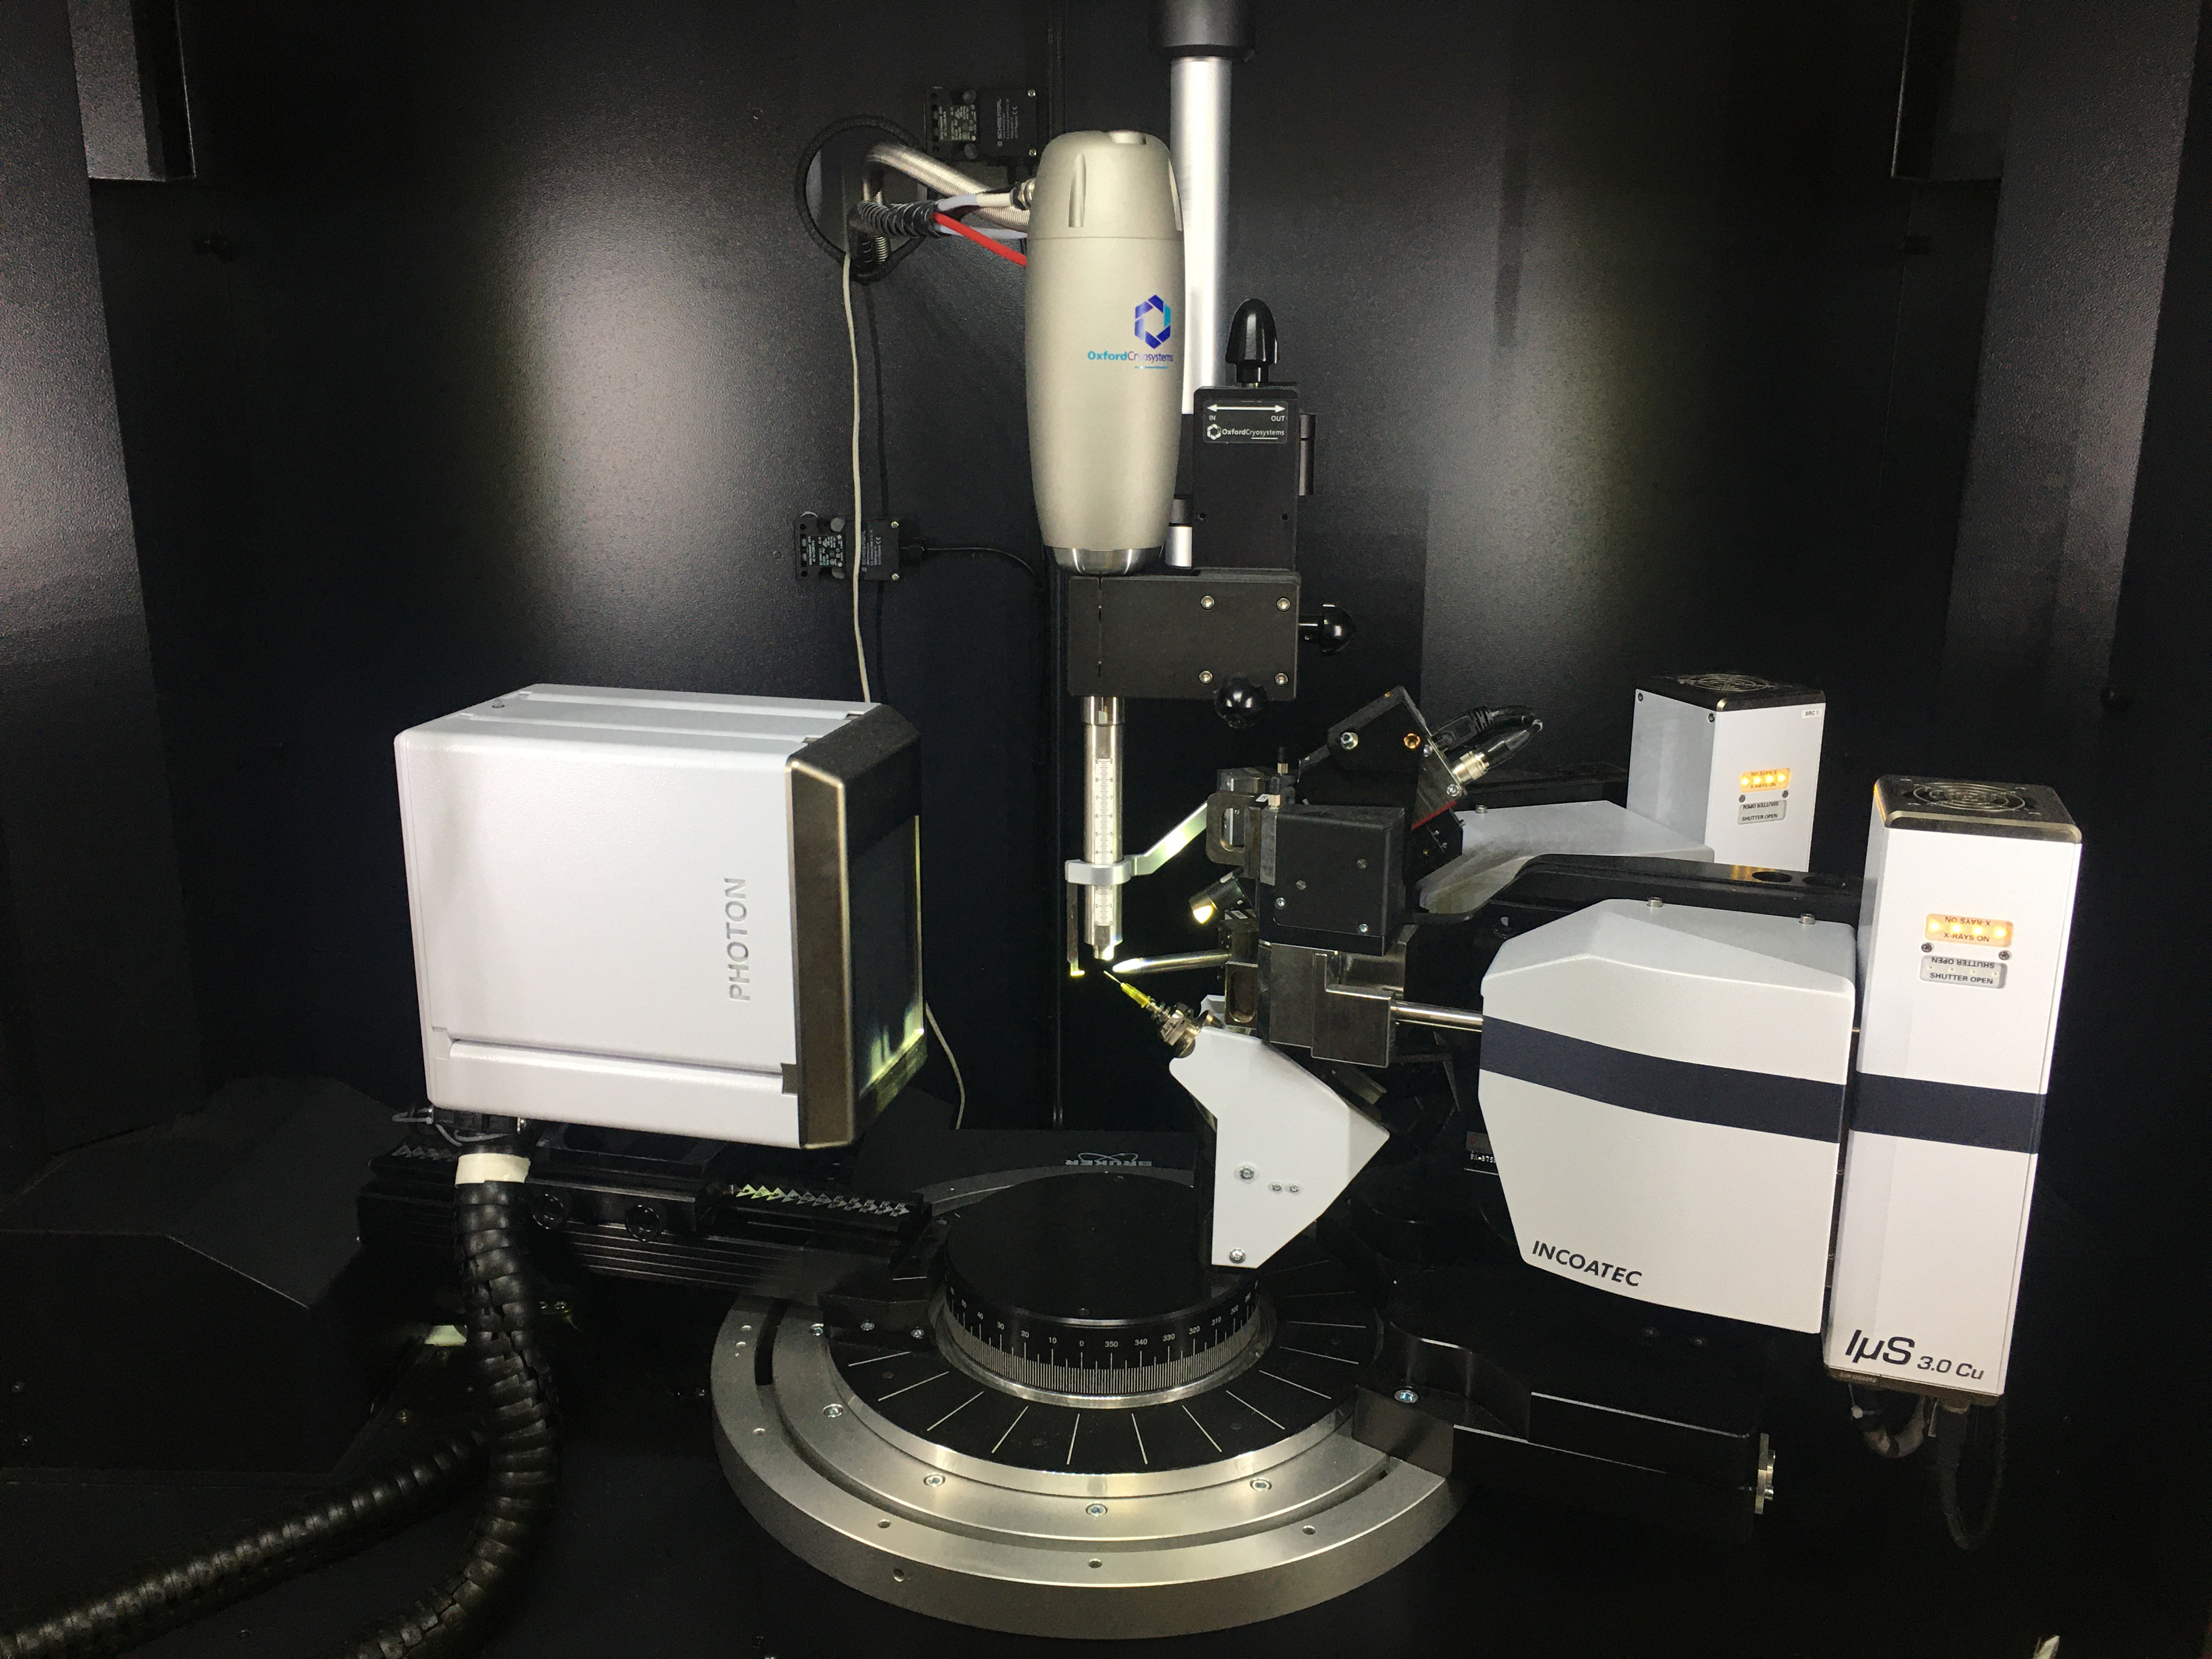
\includegraphics[width=0.8\textwidth]{d8_3.jpeg}
    \caption{Фотография установки}%
    \label{fig:D8_photo}
\end{figure}

\subsection{Исследуемые образцы}
Для определения точности методики были использованы эталонные монокристаллы Si и Ge.

Монокристалл Si имел линейные размеры примерно $50 \unit{мкм}$.
Он является осколком кристалла, который ранее был исследован по методу Бонда~\cite{Lisoivan:1982}.
Значение $a = 5.430933(12)\unit{\AA}$ там было получено с использованием значение длины волны $\lambda \text{Cu} K \alpha_1 = 1.540562\unit{\AA}$.
При пересчете на более точное значение из таблицы~\ref{tab:wavelengths}, эталонное значение ПЭЯ для Si
\[ a_\text{Si} = 5.431042 (12)\unit{\AA}. \]

Монокристалл Ge также был размером около $50 \unit{мкм}$.
Его ПЭЯ измеряли в множестве работ методами Бонда, многократных отражений и многолучевой дифракции.
Полученные при этом значения ПЭЯ~\cite{Lisoivan:1982} лежат в интервале от $5.65776 (2) \unit{\AA}$ до $5.657837 (15) \unit{\AA}$.
Из них было выбрано значение $a = 5.657772 (10) \unit{\AA}$~\cite{Cooper:1962}, так как оно оказывается наиболее близким к среднему.
Пересчет для приведенного в таблице \ref{tab:wavelengths} значения длины волны дает
\[ a_\text{Ge} = 5.657885 (10)\unit{\AA} \]

Также, с целью определения однородности продукта синтеза и значения мольной доли $x$ был изучен продукт синтеза твердого раствора оксида иттрия-европия \YEu.
Для этого было отобрано 5 различных монокристаллов, ля каждого из которых был проведен РСтА и измерение ПЭЯ по разработанной методике.

\subsection{Описание методики}

Первое описание методики дано в статье~\cite{Kudryavtsev:2024:YEu}.
Общая схема проведения измерений выглядит примерно так:
\begin{enumerate}
    \item Отбор монокристалла
    \item Предварительная съемка
    \item Выбор рефлекса
    \item Съемка рефлекса
    \item Обработка профилей
    \item Расчет межплоскостного расстояния
\end{enumerate}
\subsubsection{Отбор монокристалла}
Отбор монокристалла проводится так же, как и для РСтА.
Монокристалл выбирается так, чтобы не превосходить размера первичного пучка.
В нашем случае оптимальный размер равен приблизительно 50~мкм.
\subsubsection{Предварительная съемка}
Предварительная съемка проводится с целью определения ориентации кристалла, его дифракционного класса и получения данных об интенсивности рефлексов.

Сама съемка состоит серии полных сканирований при вращении вокруг оси $\varphi$ с шагом $0.5\degree$ для при фиксированном угле $\omega$.
Три таких сканирования выполняются при углах детектора $2\theta_D = \{-45\degree, 0\degree, 45\degree\}$ при фиксированном расстоянии до образца $D \approx 70\unit{мм}$.

Обработка снимков и получение ориентации производится в программе APEX3.
На выходе программы получается файл формата p4p, где информация об ориентации кристалла содержится в виде UB матрицы~\cite{Busing:1967}.

\subsubsection{Выбор рефлекса}
Выбор рефлекса для съемки происходит так, чтобы погрешность измерений была минимальной.
Основными критериями в таком случае оказываются наибольшие угол $2\theta$ и интенсивность рефлекса.
При этом необходимо учитывать геометрию установки, так как не все рефлексы оказывается возможно вывести в отражающее положение для двух симметричных положений в экваториальной плоскости.

Средствами программы APEX3 производить такой перебор рефлексов неэффективно и крайне проблематично, так как программа рассчитывает для одного рефлекса максимум только одну пару углов $(\varphi, \omega)$ из двух возможных в общем случае.
Поэтому была специально написана программа~\cite{Kudryavtsev:2024:eccentr} для перебора всех рефлексов, расчета для них углов гониометра и отбора случаев когда в оказывается возможным вывести рефлекс в два симметричных положения, а также когда доступна для выведения и его фриделевская пара.

Программа позволяет находить среди множества плоскостей, связанных симметрией такие, которые можно вывести в отражающее положение хотя бы при одном (из двух симметричных) положений детектора.
Для этого используется информация о текущей ориентации кристалла на гониометре, т.е. p4p-файл, в котором находится матрица ориентации UB и предварительные значения ПЭЯ.
Используя известную длину волны, размеры пикселя, расстояние до детектора, и другие неизменные параметры прибора, программа вычисляет углы гониометра $(\varphi, \omega)$, необходимые для выведения каждой плоскости в отражающее положение на экваториальную плоскость.
В каждом случае проверяются геометрические ограничения прибора.
Полученная информация для всех подходящих рефлексов собирается в таблицу Excel, ее можно проанализировать и провести отбор.
\subsubsection{Съемка рефлекса}
Съемка рефлекса представляет собой сканирование при вращении вокруг оси $\omega$ в диапазоне $\pm 2\degree$ относительно рассчитанного значения $\omega$ для отражающего положения.
Время съемки выставлялось таким, чтобы максимум на профиле пика составлял не менее 10000~имп.

В программе APEX3 невозможно выставить время съемки больше, чем 600~с, поэтому для достижения последнего условия производились несколько одинаковых съемок, пока не была достигнута требуемая интенсивность.
\subsubsection{Обработка профилей}
Обработка профилей состоит из нескольких этапов, по завершению которых можно рассчитать межплоскостное расстояние.
Реализована она была тоже в виде программы~\cite{Kudryavtsev:2024:eccentr}.

На входе она использует p4p-файл и информацию о примерном положении центра детектора (результат юстировки, прямое определение, калибровка).
Из экспериментального фрейма вырезается центральная область $X = \pm 30\unit{пикс.}, Y = \pm 15\unit{пикс.}$, в которой, исходя из условия $2\theta_D \approx 2\theta$, должен находиться искомый рефлекс.
Медианное значение интенсивности принимается за начальное значение фона.
Пиксели с интенсивностью больше заранее заданной принимаются за ''горячие пиксели'' и их значения приравниваются среднему значению по 8 соседним пикселям.
После учета горячих пикселей максимум интенсивности в выбранной области назначается примерным положением $K\alpha_1$--составляющей.
Далее, исходя из значений $D$ и $2\theta$ рассчитывается положение $K\alpha_1$--составляющей и обе точки смещаются так, чтобы теоретическое положение $K\alpha_1$ совпадало с координатами найденного максимума интенсивности.
Аппроксимация дублета проводится двумя независимыми  функциями 2D-Gauss, т.е. без закрепления междублетного расстояния и соотношения интенсивностей составляющих $2/1$.
Направлениями главных осей берутся вдоль координат детектора $X$ и $Y$ детектора.
В наших экспериментах именно функция 2D-Gauss наиболее хорошо описывала форму пика при минимальном числе уточняемых параметров: координаты максимума, полуширины (ширина на половине высоты, FWHM) в направлениях $X$ и $Y$, и интегральная интенсивность.

\subsubsection{Рассчет межплоскостного расстояния}
Для достаточно малой разницы координат рефлексов искомый угол дифракции можно рассчитать по формуле
\begin{equation} \label{eq:bond2}
    2\theta = 2\theta_D - \frac{\gamma}{2} (X_{+} - X_{-}),
\end{equation}
где $\gamma$ --- угловой размер пикселя в точке детектирования рефлекса, $X_{-}, X_{+}$ --- координаты рефлексов при отрицательном и положительном углах детектора.
В формуле $2\theta_D$ предполагается положительным.
Знак перед разницей координат рефлексов зависит от направления координаты $X$ детектора и направлением положительного вращения детектора вокруг оси $2\theta_D$.
Если они направлены в разные стороны, то знак ``$-$'', если в одну, то ``$+$''.
В нашей установке направления выбраны так, что перед разницей должен быть ``$-$''.
\subsection{Учет эксцентриситета}
Дополнительная съемка фриделевских пар позволяет учитывать эффект смещения кристалла при вращении вокруг оси $\omega$.
Так как рефлекс при съемке выводится в экваториальную плоскость, то угол $\omega$ для фриделевской пары изначального рефлекса отличается на $180\degree$.
Так как при повороте на $180\degree$ положение кристалла как бы отражается относительно оси $\omega$, то среднее значение координат рефлексов в этих двух положения будет соответствовать положению кристалла ровно на оси $\omega$~\ref{fig:eccentr}.

\begin{figure}[ht!]
    \centering
    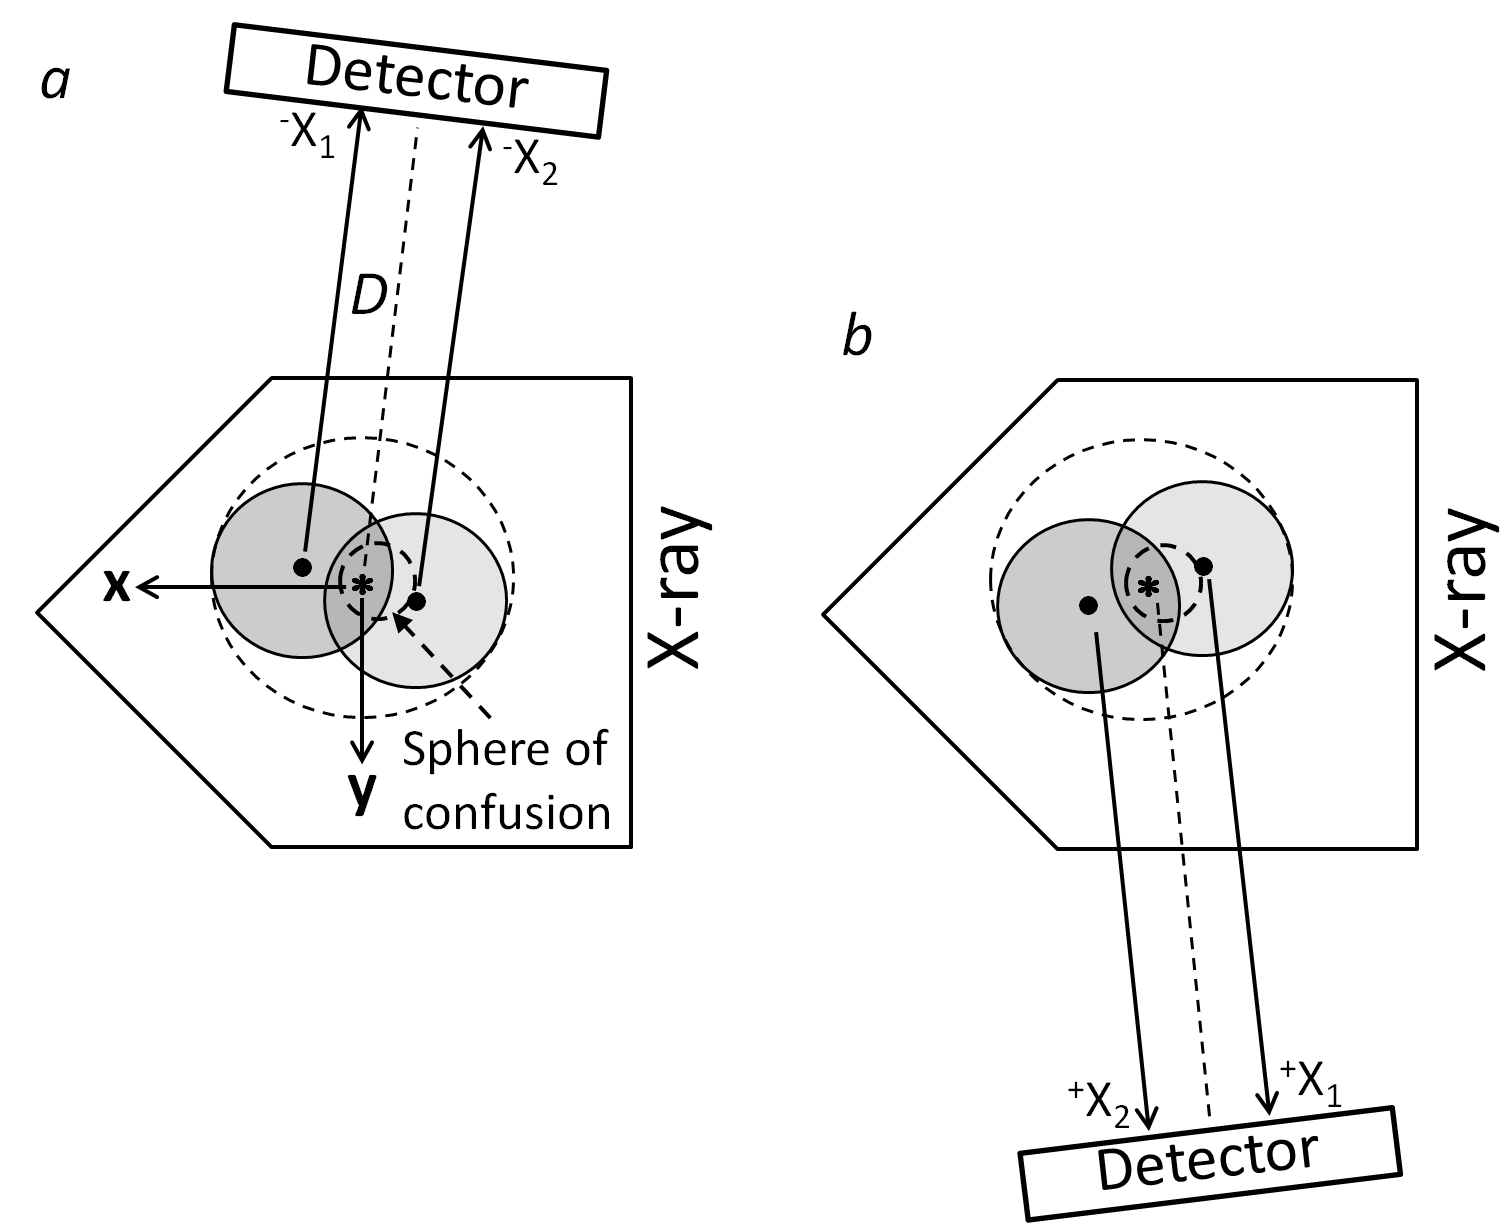
\includegraphics[width=0.8\textwidth]{eccentr.png}
    \caption{Схемы эксперимента для учета эксцентриситета образца.}\label{fig:eccentr}
\end{figure}

Таким образом измерение фриделевской пары позволяет использовать уточненное значение координат рефлекса
\[X_{true} = \frac{1}{2}(X + X_{frid})\]
где $X, X_{frid}$ --- координаты обычного рефлекса и его фриделевской пары соответственно.
Подставляя это в формулу~\ref{eq:bond2} получим
\begin{equation} \label{eq:bond4}
    2\theta = 2\theta_D - \frac{\gamma}{4} (X_{+} + X_{+frid} - X_{-} - X_{-frid}).
\end{equation}
\subsection{Расчет углового размера пикселя}
Зная линейные размеры пикселя $P$ и расстояние до центра детектора $D$ можно с хорошей точностью рассчитать угловой размер пикселя как
\begin{equation} \label{eq:gamma_simple}
    \gamma = \frac{P}{D}.
\end{equation}
В нашем случае $P = 135\unit{мкм}$, а расстояние $D$, указываемое прибором $D = 128.53\unit{мм}$.

Однако значение $D$, которое показывает прибор, всегда можно поставить под сомнение.
Правильнее провести калибровку положения детектора, например, согласно методике~\cite{Panchenko:2023}.
Для этого съемка эталонного монокристалла Si была проведена путем $\omega$--сканирования интервалов $10\degree$ в области углов $200\degree$ при пяти положениях кристалла по углу $\varphi$ (шаг $10\degree$).
Обработка полученных фреймов проведена по программе SearchXY~\cite{Panchenko:2023}.
В результате получено значение $D = 128.21\unit{мм}$.
Развороты детектора в наших экспериментах можно не учитывать из-за их малости и так как регистрация рефлексов проводится центральной областью детектора.

Полная калибровка занимает достаточно много времени и не всегда целесообразна.
Другой подход к определению $\gamma$ основан на съемке одного и того же рефлекса при двух угловых положениях детектора.
Так, рефлекс $\hkl(11 3 1)$ эталонного монокристалла Si был отснят при $2\theta_D = 96.4\degree, 97.0\degree$.
Смещение рефлекса $\Delta X$ позволяет провести вычисление $\gamma$ по формуле
\begin{equation} \label{eq:gamma_delta}
    \gamma = \frac{\Delta 2\theta_D}{\Delta X}
\end{equation}

Отметим, что такой подход позволяет проводить измерения при минимальных отклонениях рефлекса от центра детектора.
Полученное значение идеально совпадает с результатом, полученным по результатам полной калибровки.
Итоговое значение, использовавшееся далее
\[ \gamma = 0.06033\degree \]